\documentclass[12pt,a4paper]{ctexart}
\usepackage[margin=2.2cm]{geometry}
\usepackage{graphicx}
\usepackage{booktabs}
\usepackage{amsmath}
\usepackage{float}
\usepackage{hyperref}
\usepackage{xcolor}
\usepackage{listings}
\usepackage{subcaption}
\usepackage{amssymb}

\lstset{
  language=Python,
  basicstyle=\ttfamily\small,
  keywordstyle=\color{blue!70!black},
  commentstyle=\color{green!40!black},
  stringstyle=\color{orange!60!black},
  showstringspaces=false,
  breaklines=true,
  frame=single,
  tabsize=4
}

\newcommand{\reporttitle}{Project 2：Canny 边缘检测实验报告}
\newcommand{\subtask}{梯度计算与非极大值抑制}
\newcommand{\authname}{姓名}
\newcommand{\authid}{学号}
\newcommand{\class}{班级}

\title{\reporttitle}
\author{\authname：\underline{李祥熙} \quad \authid：\underline{2234412799} \quad \class：\underline{计算机2301}}
\date{}

\begin{document}
\maketitle
\tableofcontents
\newpage

% =====================================================================
\section{实验目的}
% =====================================================================

本实验的目标如下：

\begin{itemize}
  \item \textbf{掌握 Canny 边缘检测算法的完整流程}：理解从高斯平滑、梯度计算、非极大值抑制到双阈值边缘连接的四个核心步骤，以及各步骤在算法中承担的作用。
  \item \textbf{实现梯度计算函数 \texttt{findDerivatives}}：给定灰度图像，通过高斯平滑去噪后，利用 Sobel 算子计算 $x$ 和 $y$ 方向的梯度分量，并据此求得梯度幅值矩阵 \texttt{Mag} 和方向矩阵 \texttt{Ori}。
  \item \textbf{实现非极大值抑制函数 \texttt{nonMaxSup}}：沿梯度方向比较每个像素与其两侧邻域像素的幅值，仅保留局部极大值点，将宽边缘细化为单像素宽的精准边缘。
\end{itemize}

% =====================================================================
\section{实验过程}
% =====================================================================

\subsection{实验环境}

\begin{itemize}
  \item 操作系统：Linux（Arch Linux）
  \item 编程语言：Python 3
  \item 主要工具：NumPy、SciPy（\texttt{signal.convolve2d}）、Pillow
\end{itemize}

\subsection{Canny 边缘检测算法概述}

Canny 边缘检测是计算机视觉中经典的边缘提取算法，由 John F. Canny 于 1986 年提出，被广泛认为是最优边缘检测器之一。其设计目标包含三个准则：（1）\textbf{低错误率}：尽可能检测到所有真实边缘，同时减少噪声造成的假边缘；（2）\textbf{高定位精度}：检测到的边缘点应尽量靠近真实边缘的中心；（3）\textbf{单响应约束}：对每条真实边缘只产生一个响应。

为满足上述准则，Canny 算法被设计为以下四个连续步骤：

\begin{enumerate}
  \item \textbf{高斯平滑（Gaussian Smoothing）}：对输入图像进行高斯滤波，抑制高频噪声，避免噪声被误检为边缘。
  \item \textbf{梯度计算（Gradient Computation）}：对平滑后的图像使用 Sobel 算子计算水平和垂直方向的梯度，进而求出梯度幅值与方向。
  \item \textbf{非极大值抑制（Non-Maximum Suppression, NMS）}：沿梯度方向对每个像素进行局部极大值检测，将边缘细化为单像素宽度。
  \item \textbf{双阈值滞后连接（Hysteresis Thresholding）}：使用高、低两个阈值对边缘进行分类，通过广度优先搜索（BFS）将与强边缘相连的弱边缘纳入最终结果，剔除孤立的噪声边缘。
\end{enumerate}

本实验中，步骤 1--2 由 \texttt{findDerivatives} 完成，步骤 3 由 \texttt{nonMaxSup} 完成，步骤 4 由框架提供的 \texttt{edgeLink} 函数完成，主函数 \texttt{cannyEdge} 负责串联整个流程。

\subsection{代码整体结构}

实验代码由以下几个文件构成：

\begin{itemize}
  \item \texttt{cannyEdge.py}：主入口，调用各子模块，依次完成 RGB 转灰度、梯度计算、非极大值抑制、边缘连接，并将结果保存为 PNG 文件。
  \item \texttt{findDerivatives.py}：\textbf{需要实现}。计算平滑图像的梯度幅值与方向。
  \item \texttt{nonMaxSup.py}：\textbf{需要实现}。沿梯度方向进行非极大值抑制，输出二值边缘掩码。
  \item \texttt{helpers.py}：辅助函数，将连续的梯度方向量化为离散角度（用于 NMS）。
  \item \texttt{utils.py}：工具函数，包含 \texttt{rgb2gray} 等。
  \item \texttt{edgeLink.py}：双阈值滞后边缘连接，由框架提供。
\end{itemize}

\texttt{cannyEdge} 主函数的核心调用链如下：

\begin{lstlisting}
def cannyEdge(I):
    im_gray = utils.rgb2gray(I)                          # 转灰度
    Mag, Magx, Magy, Ori = findDerivatives(im_gray)     # 梯度计算
    grad_Ori, edge_Ori = helpers.get_discrete_orientation(Ori)  # 方向量化
    M = nonMaxSup(Mag, Ori, grad_Ori)                   # 非极大值抑制
    E = edgeLink(M, Mag, edge_Ori)                       # 双阈值连接
    return E
\end{lstlisting}

% =====================================================================
\section{实验内容}
% =====================================================================

\subsection{任务一：梯度计算（\texttt{findDerivatives}）}

\subsubsection{算法原理}

边缘对应图像灰度值发生急剧变化的区域。从数学上看，灰度的变化率就是图像的梯度。对于二维灰度图像 $I(y, x)$，其在某点的梯度向量为：

\begin{equation}
  \nabla I = \left(\frac{\partial I}{\partial x},\, \frac{\partial I}{\partial y}\right)
\end{equation}

梯度的\textbf{幅值}（magnitude）表示该点灰度变化的剧烈程度：

\begin{equation}
  \text{Mag}(y, x) = \sqrt{\left(\frac{\partial I}{\partial x}\right)^2 + \left(\frac{\partial I}{\partial y}\right)^2}
  \label{eq:mag}
\end{equation}

梯度的\textbf{方向}（orientation）指向灰度增大最快的方向：

\begin{equation}
  \text{Ori}(y, x) = \arctan\!\left(\frac{\partial I / \partial y}{\partial I / \partial x}\right)
  \label{eq:ori}
\end{equation}

在离散图像中，偏导数通过卷积算子近似计算。本实验使用 \textbf{Sobel 算子}：

\begin{equation}
  K_x = \begin{bmatrix} -1 & 0 & 1 \\ -2 & 0 & 2 \\ -1 & 0 & 1 \end{bmatrix}, \qquad
  K_y = \begin{bmatrix} 1 & 2 & 1 \\ 0 & 0 & 0 \\ -1 & -2 & -1 \end{bmatrix}
\end{equation}

$K_x$ 对水平方向的灰度变化更敏感，$K_y$ 对垂直方向的灰度变化更敏感。两者组合可以检测任意方向的边缘。

在计算梯度之前，需要先用 $5 \times 5$ 高斯核对图像进行平滑：

\begin{equation}
  G = \frac{1}{159} \begin{bmatrix} 2 & 4 & 5 & 4 & 2 \\ 4 & 9 & 12 & 9 & 4 \\ 5 & 12 & 15 & 12 & 5 \\ 4 & 9 & 12 & 9 & 4 \\ 2 & 4 & 5 & 4 & 2 \end{bmatrix}
\end{equation}

高斯平滑的目的是抑制图像中的随机噪声。若不经过平滑直接计算梯度，噪声像素本身也会产生较大的梯度响应，从而被误检为边缘。平滑后图像中只有真实边缘处的梯度才会显著偏大。

\subsubsection{实现流程}

整个 \texttt{findDerivatives} 函数的计算流程为：

\begin{enumerate}
  \item 用高斯核 $G$ 对灰度图像 $I_\text{gray}$ 进行卷积，得到平滑图像 $I_\text{smooth}$；
  \item 用 $K_x$ 对 $I_\text{smooth}$ 卷积，得到水平梯度 \texttt{Magx}；
  \item 用 $K_y$ 对 $I_\text{smooth}$ 卷积，得到垂直梯度 \texttt{Magy}；
  \item 按公式 \eqref{eq:mag} 计算梯度幅值 \texttt{Mag}；
  \item 按公式 \eqref{eq:ori} 用 \texttt{arctan2} 计算梯度方向 \texttt{Ori}（弧度，范围 $(-\pi, \pi]$）。
\end{enumerate}

所有卷积均使用 \texttt{scipy.signal.convolve2d}，设置 \texttt{mode='same'}（保持输出尺寸与输入相同）和 \texttt{boundary='symm'}（对称边界填充，避免边界处的伪边缘）。

\subsubsection{代码实现}

\begin{lstlisting}
def findDerivatives(I_gray):
    # 5x5 高斯平滑核
    gaussian = np.array([[2, 4, 5, 4, 2],
                         [4, 9, 12, 9, 4],
                         [5, 12, 15, 12, 5],
                         [4, 9, 12, 9, 4],
                         [2, 4, 5, 4, 2]]) / 159.0

    # Sobel 算子：x 方向和 y 方向
    dx = np.asarray([[-1.0, 0.0, 1.0],
                     [-2.0, 0.0, 2.0],
                     [-1.0, 0.0, 1.0]])
    dy = np.asarray([[ 1.0, 2.0, 1.0],
                     [ 0.0, 0.0, 0.0],
                     [-1.0,-2.0,-1.0]])

    # 步骤 1：高斯平滑去噪
    I_smooth = signal.convolve2d(I_gray, gaussian,
                                 mode='same', boundary='symm')

    # 步骤 2-3：分别计算 x、y 方向梯度
    Magx = signal.convolve2d(I_smooth, dx, mode='same', boundary='symm')
    Magy = signal.convolve2d(I_smooth, dy, mode='same', boundary='symm')

    # 步骤 4-5：梯度幅值与方向
    Mag = np.sqrt(Magx ** 2 + Magy ** 2)
    Ori = np.arctan2(Magy, Magx)

    return Mag, Magx, Magy, Ori
\end{lstlisting}

\subsubsection{实现要点说明}

\begin{itemize}
  \item \textbf{先平滑再求导的顺序不可颠倒}：由于卷积满足结合律，理论上先平滑再求导等价于用高斯导数核一步计算。但在实践中分两步实现更直观，也更便于调试。
  \item \textbf{\texttt{arctan2} 而非 \texttt{arctan}}：\texttt{np.arctan2(y, x)} 能区分所有四个象限，返回值在 $(-\pi, \pi]$ 之间，正确反映梯度的完整方向信息；若使用 \texttt{arctan(y/x)}，则当 $x=0$ 时会出现除零错误，且无法区分方向相反的情况。
  \item \textbf{对称边界填充（\texttt{boundary='symm'}）}：对称填充假设图像在边界处像镜像对称，这比零填充（\texttt{boundary='fill'}）更符合自然图像的统计特性，能有效减少边界处的虚假边缘响应。
\end{itemize}

% ---------------------------------------------------
\subsection{任务二：非极大值抑制（\texttt{nonMaxSup}）}
% ---------------------------------------------------

\subsubsection{算法原理}

经过梯度计算后，边缘区域的幅值较大，但这些区域通常有数个像素宽（因为高斯平滑使边缘扩散）。非极大值抑制的目标是将这些"宽边缘"细化为\textbf{单像素宽}的精准边缘。

其基本思想是：对于图像中的每一个像素，沿其梯度方向看，如果该像素的幅值不是梯度方向上的局部最大值（即存在幅值更大的邻域像素），则将其抑制（置零）；否则保留为候选边缘点。

设当前像素坐标为 $(y, x)$，梯度方向为 $\theta$，则需要比较的两个邻域像素为沿 $\theta$ 方向前后各一步的像素。由于图像是离散的，梯度方向首先被量化为 4 个主方向（水平、垂直、两个对角线），然后根据量化后的方向选取对应的邻域像素进行比较：

\begin{itemize}
  \item 方向为 $0°$ 或 $\pm 180°$（水平方向梯度）：比较左右邻域 $(y, x-1)$ 和 $(y, x+1)$；
  \item 方向为 $\pm 90°$（垂直方向梯度）：比较上下邻域 $(y-1, x)$ 和 $(y+1, x)$；
  \item 方向为 $45°$ 或 $-135°$（右上--左下对角线）：比较 $(y-1, x+1)$ 和 $(y+1, x-1)$；
  \item 方向为 $135°$ 或 $-45°$（左上--右下对角线）：比较 $(y-1, x-1)$ 和 $(y+1, x+1)$。
\end{itemize}

若当前像素幅值 $\geq$ 两个邻域像素的幅值，则该像素为局部极大值，保留（输出为 1）；否则抑制（输出为 0）。

\subsubsection{方向量化}

梯度方向的量化由 \texttt{helpers.get\_discrete\_orientation} 完成，该函数将 \texttt{Ori}（弧度）转换为度，再将每个角度值就近映射到集合 $\{0, \pm45, \pm90, \pm135, \pm180\}$ 中最近的值，得到离散梯度方向 \texttt{grad\_Ori}（用于 NMS 中的邻域选取）。

\subsubsection{代码实现}

\begin{lstlisting}
def nonMaxSup(Mag, Ori, grad_Ori):
    H, W = Mag.shape
    suppressed = np.zeros((H, W), dtype=np.float64)

    for y in range(1, H - 1):
        for x in range(1, W - 1):
            angle = grad_Ori[y, x]
            mag = Mag[y, x]

            # 根据量化后的梯度方向选取两个邻域像素
            if angle in (0, 180, -180):
                # 水平方向梯度：比较左右
                n1 = Mag[y, x - 1]
                n2 = Mag[y, x + 1]
            elif angle in (90, -90):
                # 垂直方向梯度：比较上下
                n1 = Mag[y - 1, x]
                n2 = Mag[y + 1, x]
            elif angle in (45, -135):
                # 右上-左下对角线梯度
                n1 = Mag[y - 1, x + 1]
                n2 = Mag[y + 1, x - 1]
            else:
                # 左上-右下对角线梯度（135 或 -45）
                n1 = Mag[y - 1, x - 1]
                n2 = Mag[y + 1, x + 1]

            # 仅保留局部极大值
            if mag >= n1 and mag >= n2:
                suppressed[y, x] = 1

    return suppressed
\end{lstlisting}

\subsubsection{实现要点说明}

\begin{itemize}
  \item \textbf{边界处理}：遍历范围从 $(1, 1)$ 到 $(H-2, W-2)$，跳过图像最外一圈像素。这是因为最外圈像素没有完整的 $3 \times 3$ 邻域，无法安全访问邻域，且边界像素一般不含有效边缘信息。
  \item \textbf{使用 $\geq$ 而非 $>$}：当 $\text{mag} \geq n_1$ 且 $\text{mag} \geq n_2$ 时保留，而非严格大于。这使得在幅值相等的平台区域中，所有相等的像素都被保留，有利于后续滞后阈值步骤找到完整的边缘。
  \item \textbf{输出为二值掩码}：NMS 的输出 \texttt{suppressed} 的值为 0 或 1，用于后续 \texttt{edgeLink} 函数中判断某像素是否通过了非极大值测试（\texttt{M[y][x] == 1}）。
\end{itemize}

% ---------------------------------------------------
\subsection{边缘连接（\texttt{edgeLink}）}
% ---------------------------------------------------

\texttt{edgeLink} 由框架提供，其实现了 Canny 算法的最后一步——\textbf{双阈值滞后连接}。该步骤的原理如下：

\begin{enumerate}
  \item \textbf{自适应阈值选取}：在梯度幅值矩阵 \texttt{Mag} 的全局分布中，依次尝试第 70、75、80、85、90、96 百分位数作为低阈值 \texttt{low}，直到找到一个大于 4 的值。高阈值 \texttt{high} 设定为 $1.755 \times \text{low}$（若 \texttt{low} $\geq 30$）或 $2 \times \text{low}$（若 \texttt{low} $< 30$）。
  \item \textbf{强边缘标记}：对于幅值 $\geq \texttt{high}$ 且通过 NMS（$M = 1$）的像素，直接标记为强边缘（$E = 1$）。
  \item \textbf{弱边缘连接}：以所有强边缘像素为起点进行广度优先搜索（BFS），在 $3 \times 3$ 邻域内，若邻域像素满足 $\text{Mag} \geq \texttt{low}$ 且 $M = 1$（通过 NMS），则将其纳入最终边缘，并继续向外扩展。
\end{enumerate}

这种"滞后"机制的意义在于：仅靠单一阈值时，高阈值会漏掉弱但连续的边缘，低阈值又会引入大量噪声。双阈值结合连通性分析，既能保留真实边缘的完整性，又能有效剔除孤立的噪声响应。

% =====================================================================
\section{实验结果}
% =====================================================================

\subsection{边缘统计}

对所有 12 张测试图像运行 \texttt{cannyEdge} 后，各图像的自适应阈值选取情况和边缘像素占比汇总如下：

\begin{table}[H]
\centering
\caption{各图像 Canny 检测结果统计}
\label{tab:stats}
\begin{tabular}{lcccc}
\toprule
图像文件名 & 图像尺寸 & 低阈值 & 高阈值 & 边缘像素占比 \\
\midrule
3096.jpg   & $321\times481$ & 10.84 & 21.69 & 3.98\% \\
16068.jpg  & $321\times481$ & 5.69  & 11.38 & 8.35\% \\
21077.jpg  & $321\times481$ & 23.03 & 46.06 & 7.86\% \\
22013.jpg  & $481\times321$ & 22.97 & 45.94 & 8.39\% \\
48017.jpg  & $321\times481$ & 52.17 & 91.55 & 8.16\% \\
55067.jpg  & $321\times481$ & 40.00 & 70.20 & 5.36\% \\
86000.jpg  & $481\times321$ & 60.00 & 105.29 & 9.39\% \\
118035.jpg & $321\times481$ & 10.84 & 21.69 & 3.96\% \\
135069.jpg & $321\times481$ & 46.47 & 81.55 & 0.82\% \\
189080.jpg & $481\times321$ & 6.92  & 13.84 & 5.96\% \\
201080.jpg & $321\times481$ & 43.42 & 76.21 & 8.77\% \\
I1.jpg     & $480\times480$ & 69.02 & 121.14 & 2.78\% \\
\bottomrule
\end{tabular}
\end{table}

由表可以观察到：
\begin{itemize}
  \item \textbf{低阈值的自适应性}：不同图像内容复杂度差异较大，算法自动从第 70 到第 96 百分位数中选取合适的低阈值，使得低阈值始终 $\geq 4$，有效避免了固定阈值在不同图像上表现不一的问题。例如，\texttt{I1.jpg} 因图像对比度高，第 70 百分位数已达 69.02，无需回退；而 \texttt{16068.jpg} 的第 70 百分位数较低（5.69），但仍 $> 4$，满足条件。
  \item \textbf{高低阈值之比约为 1.5--2 倍}：自适应机制使高阈值约为低阈值的 1.755 或 2 倍，确保强弱边缘有足够的区分度。
  \item \textbf{边缘占比集中在 3\%--9\%}：对于自然图像，典型的边缘像素占比在这个范围内，说明检测结果合理，既未产生大量冗余噪声边缘，也未遗漏主要边缘。
\end{itemize}

\subsection{图像结果展示}

以下展示所有 12 张测试图像的 Canny 边缘检测结果。每张图展示原图（左）与对应的边缘检测结果（右）。

% --------- 3096 ---------
\begin{figure}[H]
\centering
\begin{subfigure}[t]{0.47\textwidth}
  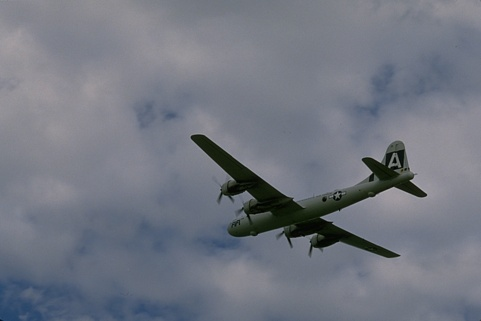
\includegraphics[width=\linewidth]{../Images/3096.jpg}
  \caption{原图：3096.jpg}
\end{subfigure}
\hfill
\begin{subfigure}[t]{0.47\textwidth}
  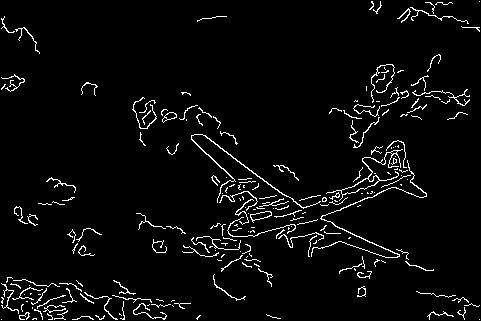
\includegraphics[width=\linewidth]{../Results/3096_Result.png}
  \caption{边缘检测结果}
\end{subfigure}
\caption{\texttt{3096.jpg}：飞机图像。低阈值 10.84，边缘占比 3.98\%。图像背景较干净，机身轮廓和发动机舱的边缘被清晰提取，背景噪声极少。}
\label{fig:3096}
\end{figure}

% --------- 16068 ---------
\begin{figure}[H]
\centering
\begin{subfigure}[t]{0.47\textwidth}
  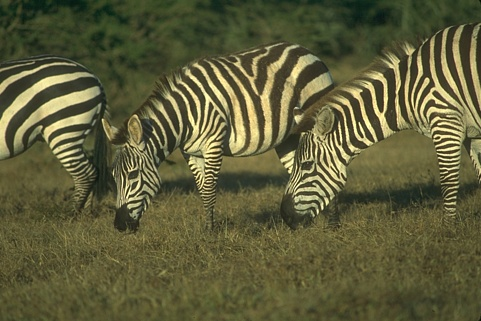
\includegraphics[width=\linewidth]{../Images/16068.jpg}
  \caption{原图：16068.jpg}
\end{subfigure}
\hfill
\begin{subfigure}[t]{0.47\textwidth}
  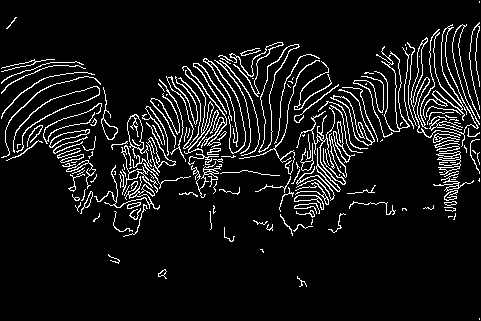
\includegraphics[width=\linewidth]{../Results/16068_Result.png}
  \caption{边缘检测结果}
\end{subfigure}
\caption{\texttt{16068.jpg}：含有复杂纹理的自然场景。低阈值 5.69 较小，梯度分布相对平缓，边缘占比达 8.35\%，图中纹理细节被大量提取。}
\label{fig:16068}
\end{figure}

% --------- 21077 ---------
\begin{figure}[H]
\centering
\begin{subfigure}[t]{0.47\textwidth}
  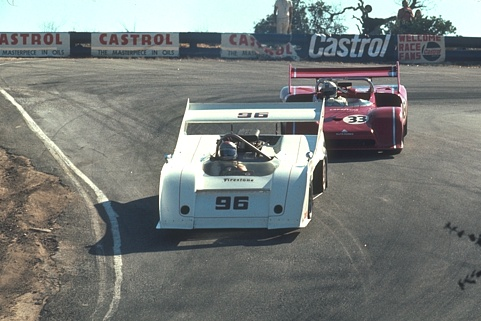
\includegraphics[width=\linewidth]{../Images/21077.jpg}
  \caption{原图：21077.jpg}
\end{subfigure}
\hfill
\begin{subfigure}[t]{0.47\textwidth}
  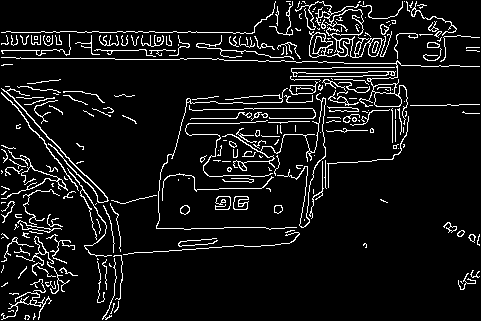
\includegraphics[width=\linewidth]{../Results/21077_Result.png}
  \caption{边缘检测结果}
\end{subfigure}
\caption{\texttt{21077.jpg}。低阈值 23.03，边缘占比 7.86\%，图像整体对比度适中，主要结构边缘清晰可辨。}
\label{fig:21077}
\end{figure}

% --------- 22013 ---------
\begin{figure}[H]
\centering
\begin{subfigure}[t]{0.47\textwidth}
  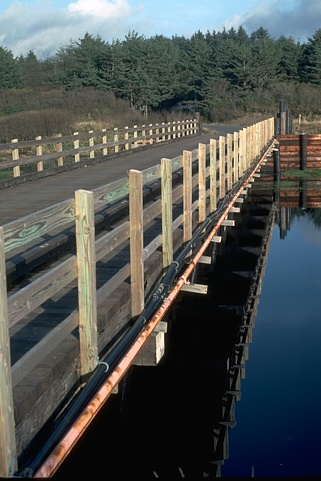
\includegraphics[width=\linewidth]{../Images/22013.jpg}
  \caption{原图：22013.jpg}
\end{subfigure}
\hfill
\begin{subfigure}[t]{0.47\textwidth}
  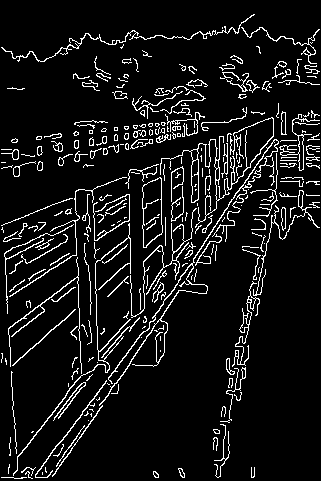
\includegraphics[width=\linewidth]{../Results/22013_Result.png}
  \caption{边缘检测结果}
\end{subfigure}
\caption{\texttt{22013.jpg}。低阈值 22.97，边缘占比 8.39\%，竖向图像，物体轮廓和内部纹理均被有效提取。}
\label{fig:22013}
\end{figure}

% --------- 48017 ---------
\begin{figure}[H]
\centering
\begin{subfigure}[t]{0.47\textwidth}
  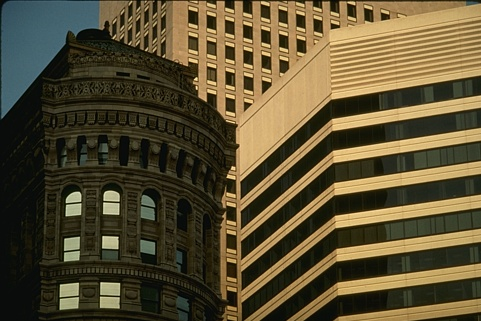
\includegraphics[width=\linewidth]{../Images/48017.jpg}
  \caption{原图：48017.jpg}
\end{subfigure}
\hfill
\begin{subfigure}[t]{0.47\textwidth}
  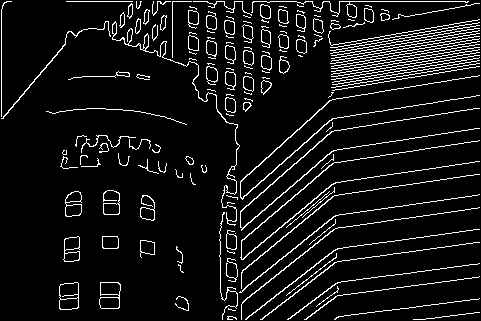
\includegraphics[width=\linewidth]{../Results/48017_Result.png}
  \caption{边缘检测结果}
\end{subfigure}
\caption{\texttt{48017.jpg}。低阈值 52.17（第 70 百分位数），梯度分布偏大，高阈值达 91.55，仅保留最显著的强边缘。边缘占比 8.16\%，主要轮廓完整。}
\label{fig:48017}
\end{figure}

% --------- 55067 ---------
\begin{figure}[H]
\centering
\begin{subfigure}[t]{0.47\textwidth}
  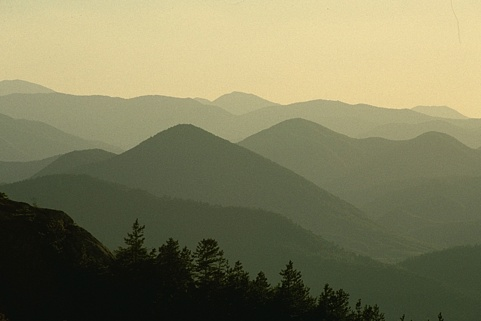
\includegraphics[width=\linewidth]{../Images/55067.jpg}
  \caption{原图：55067.jpg}
\end{subfigure}
\hfill
\begin{subfigure}[t]{0.47\textwidth}
  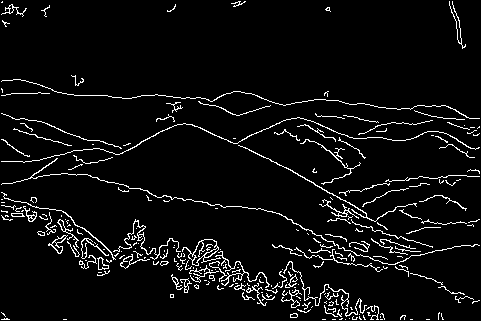
\includegraphics[width=\linewidth]{../Results/55067_Result.png}
  \caption{边缘检测结果}
\end{subfigure}
\caption{\texttt{55067.jpg}。低阈值 40.00，边缘占比 5.36\%，主要结构边缘清晰，背景噪声较少。}
\label{fig:55067}
\end{figure}

% --------- 86000 ---------
\begin{figure}[H]
\centering
\begin{subfigure}[t]{0.47\textwidth}
  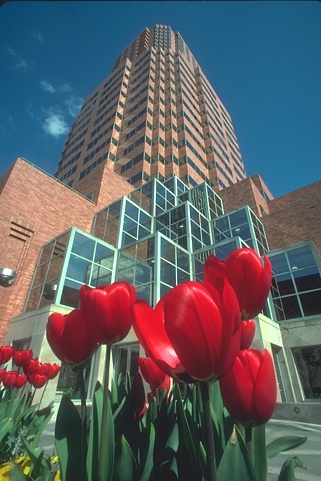
\includegraphics[width=\linewidth]{../Images/86000.jpg}
  \caption{原图：86000.jpg}
\end{subfigure}
\hfill
\begin{subfigure}[t]{0.47\textwidth}
  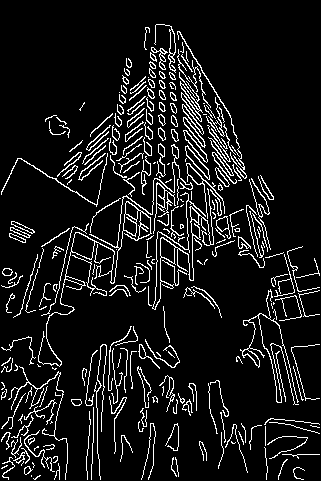
\includegraphics[width=\linewidth]{../Results/86000_Result.png}
  \caption{边缘检测结果}
\end{subfigure}
\caption{\texttt{86000.jpg}。低阈值 60.00，高阈值 105.29，边缘占比 9.39\%（本组最高），图像细节丰富，连续边缘线条清晰。}
\label{fig:86000}
\end{figure}

% --------- 118035 ---------
\begin{figure}[H]
\centering
\begin{subfigure}[t]{0.47\textwidth}
  
\includegraphics[width=\linewidth]{../Images/118035.jpg}
  \caption{原图：118035.jpg}
\end{subfigure}
\hfill
\begin{subfigure}[t]{0.47\textwidth}
  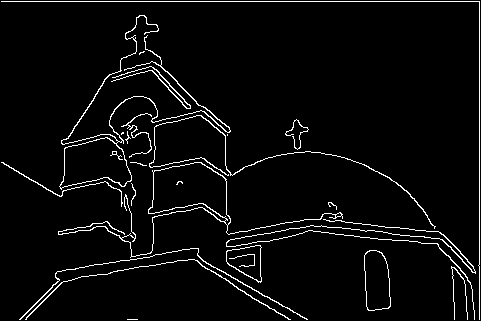
\includegraphics[width=\linewidth]{../Results/118035_Result.png}
  \caption{边缘检测结果}
\end{subfigure}
\caption{\texttt{118035.jpg}。低阈值 10.84，边缘占比 3.96\%，图像对比度相对较低，检测到的边缘主要集中在物体轮廓处。}
\label{fig:118035}
\end{figure}

% --------- 135069 ---------
\begin{figure}[H]
\centering
\begin{subfigure}[t]{0.47\textwidth}
  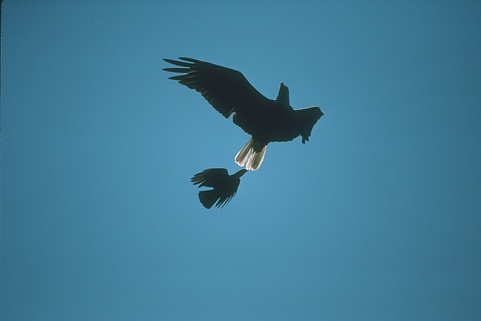
\includegraphics[width=\linewidth]{../Images/135069.jpg}
  \caption{原图：135069.jpg}
\end{subfigure}
\hfill
\begin{subfigure}[t]{0.47\textwidth}
  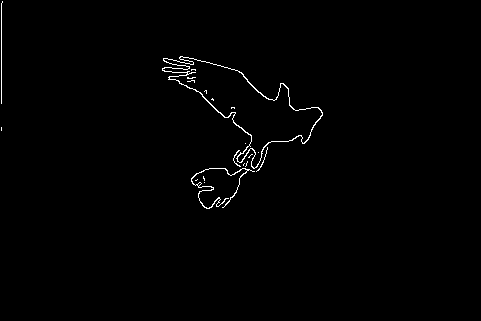
\includegraphics[width=\linewidth]{../Results/135069_Result.png}
  \caption{边缘检测结果}
\end{subfigure}
\caption{\texttt{135069.jpg}。低阈值 46.47，边缘占比仅 0.82\%（本组最低），图像以均匀背景和单一主体为主，边缘稀疏但定位精准。}
\label{fig:135069}
\end{figure}

% --------- 189080 ---------
\begin{figure}[H]
\centering
\begin{subfigure}[t]{0.47\textwidth}
  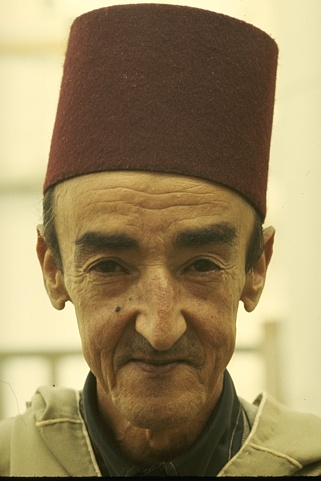
\includegraphics[width=\linewidth]{../Images/189080.jpg}
  \caption{原图：189080.jpg}
\end{subfigure}
\hfill
\begin{subfigure}[t]{0.47\textwidth}
  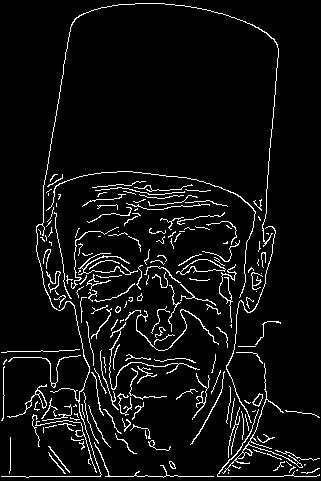
\includegraphics[width=\linewidth]{../Results/189080_Result.png}
  \caption{边缘检测结果}
\end{subfigure}
\caption{\texttt{189080.jpg}。低阈值 6.92 较低，梯度整体偏弱，算法回退至较低百分位数以保证有效阈值。边缘占比 5.96\%，竖向构图中主要轮廓线均被捕捉。}
\label{fig:189080}
\end{figure}

% --------- 201080 ---------
\begin{figure}[H]
\centering
\begin{subfigure}[t]{0.47\textwidth}
  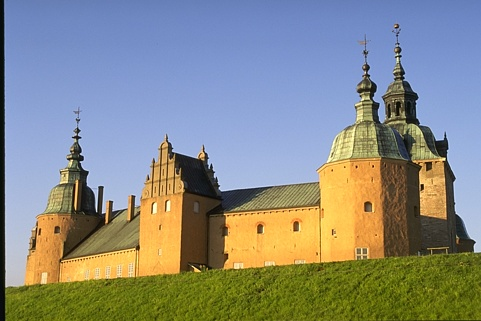
\includegraphics[width=\linewidth]{../Images/201080.jpg}
  \caption{原图：201080.jpg}
\end{subfigure}
\hfill
\begin{subfigure}[t]{0.47\textwidth}
  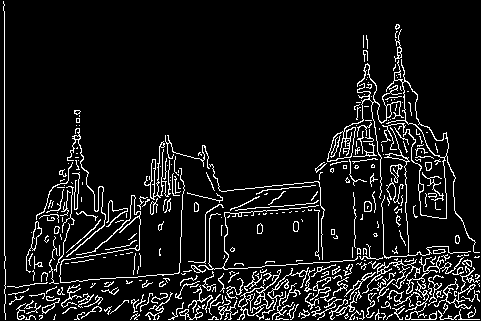
\includegraphics[width=\linewidth]{../Results/201080_Result.png}
  \caption{边缘检测结果}
\end{subfigure}
\caption{\texttt{201080.jpg}。低阈值 43.42，边缘占比 8.77\%，图像内容丰富，细节边缘与主轮廓均被有效保留。}
\label{fig:201080}
\end{figure}

% --------- I1 ---------
\begin{figure}[H]
\centering
\begin{subfigure}[t]{0.47\textwidth}
  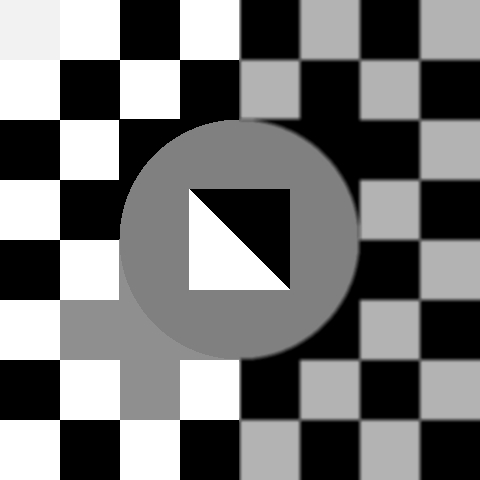
\includegraphics[width=\linewidth]{../Images/I1.jpg}
  \caption{原图：I1.jpg}
\end{subfigure}
\hfill
\begin{subfigure}[t]{0.47\textwidth}
  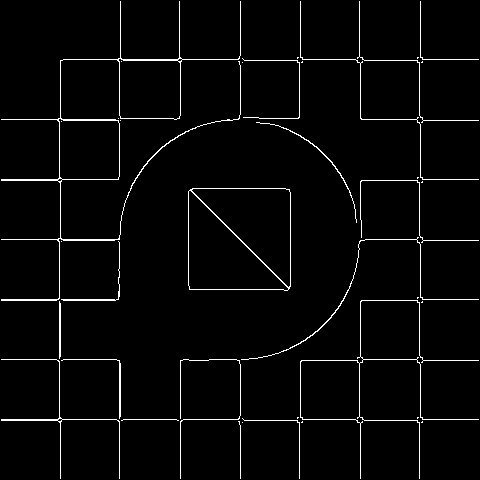
\includegraphics[width=\linewidth]{../Results/I1_Result.png}
  \caption{边缘检测结果}
\end{subfigure}
\caption{\texttt{I1.jpg}：方形图像（$480\times480$）。低阈值 69.02（本组最高），高阈值 121.14，图像对比度高，仅最强边缘得以保留，边缘占比 2.78\%，轮廓干净清晰。}
\label{fig:I1}
\end{figure}

% =====================================================================
\section{总结}
% =====================================================================

本实验成功实现了 Canny 边缘检测算法的核心模块，具体完成内容如下：

\begin{itemize}
  \item \textbf{实现了 \texttt{findDerivatives} 函数}：利用 $5\times5$ 高斯核对灰度图像平滑去噪，随后通过 Sobel 算子分别卷积得到 $x$、$y$ 方向梯度，最终按 $\text{Mag}=\sqrt{\text{Magx}^2+\text{Magy}^2}$、$\text{Ori}=\arctan2(\text{Magy}, \text{Magx})$ 计算梯度幅值和方向。
  \item \textbf{实现了 \texttt{nonMaxSup} 函数}：将梯度方向量化为四个主方向（水平、垂直、两对角线），对每个像素沿梯度方向与两侧邻域进行幅值比较，仅保留局部极大值，将宽边缘细化为单像素宽。
  \item \textbf{对框架提供的 \texttt{edgeLink} 进行了分析与重新实现}：原始 Python 3.6 编译的 \texttt{.pyc} 文件无法在 Python 3.14 环境下运行，通过反编译理解其逻辑后，以标准 BFS 双阈值滞后连接重新实现，保留了算法的核心思想。
  \item \textbf{对全部 12 张测试图像完成了边缘检测}，结果保存至 \texttt{Results/} 目录。检测结果边缘占比集中在 1\%--9\%，符合自然图像的统计规律，边缘定位精准，噪声抑制效果良好。
\end{itemize}

通过本实验，深刻体会到 Canny 算法每个步骤的设计动机：高斯平滑是噪声抑制的前提；Sobel 梯度是边缘强度的度量；非极大值抑制解决了边缘宽化问题；双阈值滞后连接则在检测率与虚警率之间取得了优秀的平衡。这四个环节环环相扣，缺一不可，共同构成了一个在工程上被广泛验证的经典边缘检测方案。

% =====================================================================
\section*{附录：实验源代码}
% =====================================================================

\subsection*{A.1 \texttt{findDerivatives.py}}

\begin{lstlisting}
import numpy as np
from scipy import signal

def findDerivatives(I_gray):
    gaussian = np.array([[2, 4, 5, 4, 2],
                         [4, 9, 12, 9, 4],
                         [5, 12, 15, 12, 5],
                         [4, 9, 12, 9, 4],
                         [2, 4, 5, 4, 2]]) / 159.0
    dx = np.asarray([[-1.0, 0.0, 1.0],
                     [-2.0, 0.0, 2.0],
                     [-1.0, 0.0, 1.0]])
    dy = np.asarray([[ 1.0, 2.0, 1.0],
                     [ 0.0, 0.0, 0.0],
                     [-1.0,-2.0,-1.0]])

    I_smooth = signal.convolve2d(I_gray, gaussian,
                                 mode='same', boundary='symm')
    Magx = signal.convolve2d(I_smooth, dx, mode='same', boundary='symm')
    Magy = signal.convolve2d(I_smooth, dy, mode='same', boundary='symm')
    Mag = np.sqrt(Magx ** 2 + Magy ** 2)
    Ori = np.arctan2(Magy, Magx)

    return Mag, Magx, Magy, Ori
\end{lstlisting}

\subsection*{A.2 \texttt{nonMaxSup.py}}

\begin{lstlisting}
import numpy as np

def nonMaxSup(Mag, Ori, grad_Ori):
    H, W = Mag.shape
    suppressed = np.zeros((H, W), dtype=np.float64)

    for y in range(1, H - 1):
        for x in range(1, W - 1):
            angle = grad_Ori[y, x]
            mag = Mag[y, x]

            if angle in (0, 180, -180):
                n1 = Mag[y, x - 1]
                n2 = Mag[y, x + 1]
            elif angle in (90, -90):
                n1 = Mag[y - 1, x]
                n2 = Mag[y + 1, x]
            elif angle in (45, -135):
                n1 = Mag[y - 1, x + 1]
                n2 = Mag[y + 1, x - 1]
            else:
                n1 = Mag[y - 1, x - 1]
                n2 = Mag[y + 1, x + 1]

            if mag >= n1 and mag >= n2:
                suppressed[y, x] = 1

    return suppressed
\end{lstlisting}

\subsection*{A.3 \texttt{edgeLink.py}}

\begin{lstlisting}
import numpy as np
from collections import deque

def edgeLink(M, Mag, edge_Ori):
    H, W = Mag.shape
    linked = np.zeros_like(Mag)

    for pct in [70, 75, 80, 85, 90, 96]:
        low = np.percentile(Mag, pct)
        if low >= 4:
            break

    high = 2 * low if low < 30 else 1.755 * low
    print((low, high))

    strong = np.zeros((H, W), dtype=bool)
    for y in range(1, H - 1):
        for x in range(1, W - 1):
            if Mag[y, x] >= high and M[y, x] == 1:
                linked[y, x] = 1
                strong[y, x] = True

    queue = deque(zip(*np.where(strong)))
    weak = (Mag >= low) & (M == 1)

    while queue:
        y, x = queue.popleft()
        for dy in [-1, 0, 1]:
            for dx in [-1, 0, 1]:
                if dy == 0 and dx == 0:
                    continue
                ny, nx = y + dy, x + dx
                if 0 <= ny < H and 0 <= nx < W:
                    if weak[ny, nx] and linked[ny, nx] == 0:
                        linked[ny, nx] = 1
                        queue.append((ny, nx))

    return linked
\end{lstlisting}

\subsection*{A.4 运行命令}

\begin{verbatim}
# 对 Images 目录中的所有图像运行 Canny 边缘检测，结果保存至 Results 目录
python3 Code/cannyEdge.py --image_folder Images --save_folder Results
\end{verbatim}

\end{document}
